%% The basic ESPResSo tutorial
%%
% Writer's guide lines:
% - provide background information and references
% - do not get lost in details but maintain a nice readability
% - describe every line of the script, that contains an ESPResSo
%   command (in future tutorial, only describe new ones) 
%
%%%%%%%%%%%%%%%%%%%%%%%%%%%%%%%%%%%%%%%%%%%%%%%%%%%%%%%%%%%%%%%%%
%%%%%%%%%%%%%%%%%%%%%%%%%%%%%%%%%%%%%%%%%%%%%%%%%%%%%%%%%%%%%%%%% 
% From the brainstorming:
%
% Preknowledge:
% 
% Basic MD(simple integrator,langevin thermostat, ---basic tcl
% basic potentials, basis tutorial 1
% 
% Basis Tutorial: written in Latex
% 
% <<every line of script code should be explained>>
% 
% 1) tcl basic setting up a system
% MD, soft sphere and Lennard-Jones Fluid (argon system), 
% Units
% 
% online visualization (pdb output)
% rdf, pressure,energy,
% 
% online analysis function
% savin, readin writeout, offline analysis, statistics
% 
% Structure:
% Part1:
% 1) Prerequisits (what you should know beforehand: basic tcl knowledge,
% Here you can find more info: Allen, Tildesley: Frenkel smit,
% Rappaport, tcl tutorial,
% 
% 2) Physics of the systems (argon, soft sphere system)
% 
% 3) Algorithms (verlocity verlet, Langevin, Potentials, LJ)
% 3b) about units
% 
% Part2 
% 1) simulation script in all detail, line by line
% Initialize
% Visualize
% Simulate (with online analysis, saves for later off-line analysis,
% (Savelize (save our lives ))
% 
% 2) a new script for later
% analysis, and other helper ideas
% 
% Things to remember and take care of:
% Use the same names for variables
% 
% ====================================================================
% General Tutorial: (the next tutorials: pe_solution, cell model of one
% charged colloid, LB, ferrofluid)
% 

% basiert auf KOMA-Script scrbook-Klasse
\documentclass[11pt,a4paper,% BCOR8mm,
	       %twoside, onecolumn, openright, cleardoubleempty, %
	       %parindent,
headnosepline, footnosepline, notitlepage, %
	       %onelinecaption,
bigheadings, % bibtotoc, %tocindent, listsindent, %
	       %chapterprefix, noappendixprefix,
	       %tablecaptionbelow,
	       %pointlessnumbers, % macht Probleme (Anhang ohne Punkt, aber sonst Kapitel mit Punkt
	       % abstractoff, fleqn, leqno,
	       % openbib, origlongtable,
final]{scrreprt}

% Satzspiegel 

% wenn keine KOMA-Klasse verwendet wird, kann so der Satzspiegel
% berechnet werden
%\usepackage[DIV15,BCOR12mm,pagesize]{typearea}

% Hier knnen Seitenhoehe und -breite individuell angepasst werden
%\areaset[BCOR]{Breite}{Hohe}
% oder 
%\usepackage[a4paper,body={15.6cm,23cm},left=3cm]{geometry}

% ============================================================================

%% Grafikpakete
% Fr einfache Einbingung von Grafiken
\usepackage{graphicx}%

% Wenn man direkt mit dem pdflatex eine PDF-Datei erzeugt, sollten diese beiden
% Pakete eingebunden werden (Hyperlinks, bessere Bildschirmschriftarten usw.)
\usepackage{color}
\definecolor{mylinkcolor}{rgb}{0.5812,0.0665,0.0659} % IndianRed 
\definecolor{mycitecolor}{rgb}{0.075,0.31,0.0431} % MossGreen 
\definecolor{myurlcolor}{rgb}{0.0118,0.098,0.7412} % DarkBlue
\usepackage[pdftex,bookmarks]{hyperref}

% Druckversion
% f�r reine pdf-Dateien noch Option colorlinks hinzufgen, um Links farbig zumachen
% \usepackage[pdftex,bookmarks,bookmarksopen,citecolor={mycitecolor},%
%  linkcolor={mylinkcolor},urlcolor={myurlcolor},breaklinks=true,%
%  hypertexnames=false,hyperindex=true,encap,colorlinks]{hyperref} %

%  	\hypersetup{
%     pdftitle = {},
%     pdfauthor = {Kai Grass},
%     pdfsubject = {},
%     pdfkeywords = {},
%     pdfcreator = {},%
%     pdfproducer = {},
% 	}%

\usepackage{ae,aecompl}

% ============================================================================

%% Sprachliche Pakete
\usepackage[english]{babel}
% Neue Deutsche Rechtschreibung
%\usepackage[ngerman]{babel}
%\usepackage{ngerman} 

% Paket zur einfacheren Eingabe deutscher Umlaute
%\usepackage[applemac]{inputenc} %Mac
\usepackage[latin1]{inputenc}   %UNIX/LINUX
% \usepackage[ansinew]{inputenc}  % Windows
\usepackage[T1]{fontenc}

% ============================================================================

% Literaturverzeichnis
\usepackage[square,numbers,sort&compress]{natbib}
%\usepackage{bibmods}
%\bibpunct{(}{)}{,}{a}{}{,}
%\bibpunct{(}{)}{,}{a}{,}{;}
\setlength{\bibsep}{1ex}

% ============================================================================

% Stichwortverzeichnis
% \usepackage{makeidx}
% \makeindex

% ============================================================================

% Deutsche Zahlenkonvention (1 (Komma) 0 statt 1 (Punkt) 0)
% \usepackage{ziffer}

%% Schriftarten
\usepackage{times} % times is used to avoid bitmap fonts in PDF

%% Mathematische Packages
% Dieses Pakete definiert viele ntzliche mathematische Befehele und
% Die Option "intlimits" bewirkt, dass beim Integral die Grenzenangaben oben
% und unten erscheinen und nicht seitlich.
\usepackage[intlimits]{amsmath}
\usepackage{amsfonts}
\usepackage{amsthm}
\usepackage{mathrsfs}
\usepackage{stmaryrd}


% Diese Schriftarten ermglichen schne Mengensymbole fr natrliche Zahlen, usw.
% siehe Definition von \N, \Z usw. Dies ist Geschmackssache.
%\usepackage{bbm}
%\usepackage{dsfont}

% Subfigures
\usepackage{subfigure}

% Needed for Tabular-Umgebung
\usepackage{array}

% werden (sog. Schusterjungen und Hurenkinder vermeiden)
%\clubpenalty = 10000
%\widowpenalty = 10000

\sloppy

% Ein Paket um "kommutative Diagramme" zu erstellen. Fuer einfhrende Beispiele
% siehe xymanual.ps und xyreference.ps
%\usepackage[all]{xy}

%%%%%%%%%%%%%%%%%%% Shortcuts %%%%%%%%%%%%%%%%%%%%%%%%%%%%%%%%%%%%%%%%%%%%
%\newcommand{\N}{\mathbbm{N}}	% Natuerliche Zahlen
%\newcommand{\Z}{\mathbbm{Z}}	% Ganze Zahlen
%\newcommand{\Q}{\mathbbm{Q}}	% Rationale Zahlen
%\newcommand{\R}{\mathbbm{R}}	% Reelle Zahlen
%\newcommand{\C}{\mathbbm{C}}	% Komplexe Zahlen
%\newcommand{\one}{\mathbbm{1}}	% Einheits Eins
%
%\newcommand{\toinf}{\to\infty}				% --> oo
%\newcommand{\tozero}{\to 0}				% --> 0
%\newcommand{\ontop}[2]{\genfrac{}{}{0pt}{}{#1}{#2}}	% Aufeinander
%\newcommand{\abs}[1]{\left|#1\right|}
%\newcommand{\argmax}{\mathop{\rm arg\,max}}

% Ein Befehl, um Abbildungen einfach einheitlich zu gestalten
% Bsp: \abb{f}{\R}{\R}{x}{x^2}

%\newcommand{\abb}[5]{%
%\setlength{\arraycolsep}{0.4ex}%
%\begin{array}{rcccc}%
%#1 &:\,& #2 & \,\,\longrightarrow\,\, & #3 \\[0.5ex]%
%     & & #4 & \longmapsto & #5%
%\end{array}%
%}

%%%%%%%%%%%%%%%%%%% Theorem definitions %%%%%%%%%%%%%%%%%%%%%%%%%%%%%%%%%%
%\theoremstyle{plain}
%\newtheorem{theorem}{Theorem}[chapter]
%\newtheorem{proposition}[theorem]{Proposition}
%\newtheorem{lemma}[theorem]{Lemma}
%\newtheorem{satz}[theorem]{Satz}
%\newtheorem{korollar}[theorem]{Korollar}
%
%\theoremstyle{definition}
%\newtheorem{definition}{Definition}[chapter]
%\newtheorem{beispiel}[theorem]{Beispiel}
%\newtheorem{bemerkung}[theorem]{Bemerkung}
%
%%%%%%%%%%%%%%%%%%%%%%%%%%%%%%%%%%%%%%%%%%%%%%%%%%%%%%%%%%%%%%%%%%%%%%%%%%

% ============================================================================
% \renewcommand*{\partpagestyle}{empty}
% \renewcommand*{\partformat}{\partname~\thepart:}
%\usepackage{fancyhdr}
%%\pagestyle{headings}
%\pagestyle{fancyplain}
%%\addtolength{\headwidth}{\marginparsep}
%%\addtolength{\headwidth}{\marginparwidth}
%\renewcommand{\chaptermark}[1]{\markboth{#1}{}}
%\renewcommand{\sectionmark}[1]{\markright{\thesection\ #1}}
%%\lhead[\fancyplain{}{\bfseries\thepage}]{\fancyplain{}{\bfseries\rightmark}}
%\lhead[\fancyplain{}{\thepage}]{\fancyplain{}{\rightmark}}
%%\rhead[\fancyplain{}{\bfseries\leftmark}]{\fancyplain{}{\bfseries\thepage}}
%\rhead[\fancyplain{}{\leftmark}]{\fancyplain{}{\thepage}}
%%\chead{}
%%\rhead{\thepage}
%%\lfoot{Schnellste Pfade in geometrischen Netzwerken}
%\cfoot{}
%%\rfoot{}
%%\setlength{\headrulewidth}{0.4pt}
%%\setlength{\footrulewidth}{0.4pt}

%\usepackage[automark]{scrpage2}
%\pagestyle{scrheadings}
%\automark[section){chapter}
%\lehead[scrplain-links-gerade]{scrheadings-links-gerade}
%\cehead[scrplain-mittig-gerade]{scrheadings-mittig-gerade}
%\rehead[scrplain-rechts-gerade]{scrheadings-rechts-gerade}
%\lefoot[scrplain-links-gerade]{scrheadings-links-gerade}
%\cefoot[scrplain-mittig-gerade]{scrheadings-mittig-gerade}
%\refoot[scrplain-rechts-gerade]{scrheadings-rechts-gerade}
%\lohead[scrplain-links-ungerade]{scrheadings-links-ungerade}
%\cohead[scrplain-mittig-ungerade]{scrheadings-mittig-ungerade}
%\rohead[scrplain-rechts-ungerade]{scrheadings-rechts-ungerade}
%\lofoot[scrplain-links-ungerade]{scrheadings-links-ungerade}
%\cofoot[scrplain-mittig-ungerade]{scrheadings-mittig-ungerade}
%\rofoot[scrplain-rechts-ungerade]{scrheadings-rechts-ungerade}
%\ihead[scrplain-innen]{scrheadings-innen}
%\chead[scrplain-zentriert]{scrheadings-zentriert}
%\ifoot[scrplain-innen]{scrheadings-innen}
%\cfoot[scrplain-zentriert]{scrheadings-zentriert}
% Markierungen: \leftmark, \rightmark, \pagemark \headmark
% \manualmark \automark

% ============================================================================  

%%%%%%%%%%%%%%%%%%%%%%%%%%%%%%%%%%%%%%%%%%%%%%%%%%%%%%%%%%%%%%%%%%%%%%%%%%
\setcounter{secnumdepth}{2}
\setcounter{tocdepth}{1}
%%%%%%%%%%%%%%%%%%%%%%%%%%%%%%%%%%%%%%%%%%%%%%%%%%%%%%%%%%%%%%%%%%%%%%%%%%

%% Schriftsatz in KOMA
%\setkomafont{Element}{Befehle}
%\addtokomafont{Element}{Befehle}
%\usekomafont{Element}

%\includeonly{kapitel/sinterkeramiken, kapitel/statisch, kapitel/dynamisch, kapitel/ergebnisse, kapitel/abbildungen,
% kapitel/literatur}
%\includeonly{kapitel/titelseite2}
% ============================================================================

\usepackage{verbatim}

% The ESPResSo Logo
% how to define it such that there is a space afterwards if needed
% but not, when there is a point afterwards ????
\newcommand{\ES}{\textbf{ESPResSo}}

% How to diplay ESPResSo commands in flowing text. Larger code segments
% should be put inside boxes.
\newcommand{\EScmd}[1]{\texttt{\textbf{#1}}}

% The code block
%\newcommand{\EScode}[1]{ \parbox{0.95\textwidth}{\texttt{#1}}}
\usepackage{listings} 
\lstset{numbers=left, numberstyle=\tiny, numbersep=5pt, showspaces=false, showstringspaces=false,postbreak=\space, breakindent=5pt, breaklines}
\lstset{language=tcl, keywordstyle=\color{blue}\bfseries ,emphstyle=\color{green}, commentstyle=\color{red}\itshape }
\lstset{keywordsprefix=setmd}
\lstset{keywords=[6]{thermostat,part,inter,integrate,rescale_velocities,code_info,save_sim,writepdb,analyze,uwerr}}


\newtheorem{task}{Task}

\begin{document}
\renewcommand{\d}{\mathrm d}
\subject{ESPResSo Tutorial}
\title{The Lattice Boltzmann Method in \ES{}: Three examples } \author{ Stefan Kesselheim \thanks{\ttfamily 
kessel@icp.uni-stuttgart.de}  \and  Georg Rempfer \thanks{\ttfamily 
georg@icp.uni-stuttgart.de}}
\date{\today}
\publishers{Institute for Computational Physics, Stuttgart University}
\maketitle 
\begin{center}
  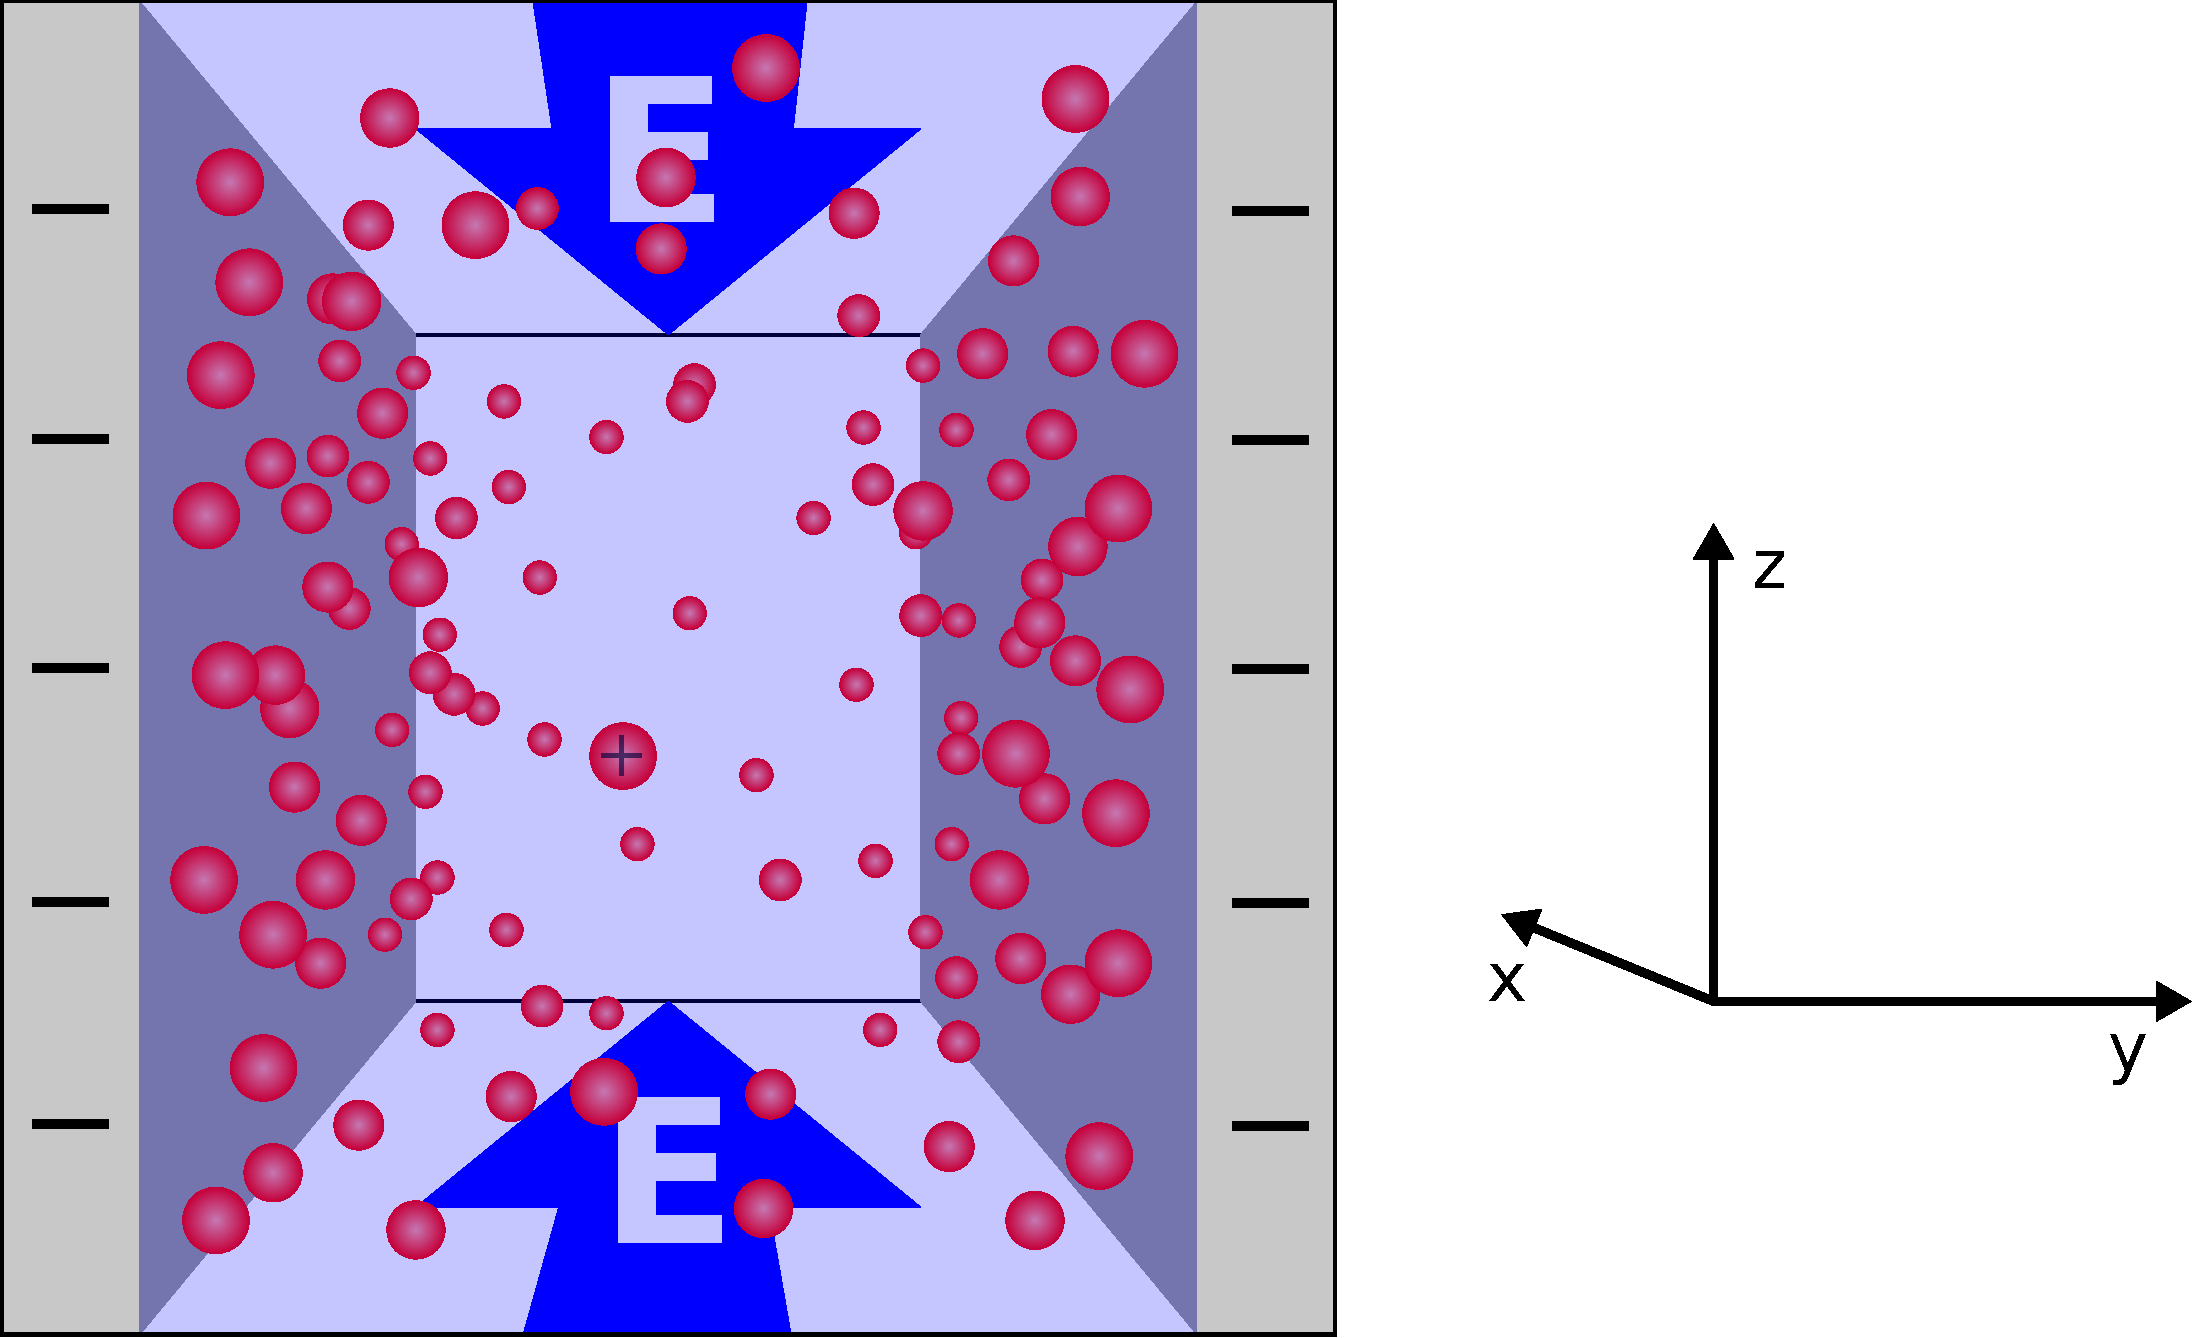
\includegraphics[width=0.5\columnwidth]{../figs/schlitzpore_3d.pdf}
\end{center}
\tableofcontents



\chapter{Introduction}
In this tutorial, you will learn basics about the 
Lattice Boltzmann Method (LBM) with special focus on the application
on soft matter simulations, or more precisely on how to apply it 
in combination with molecular dynamics to take into account 
hydrodynamic solvent effects without the need to introduce
thousands of solvent particles. 

The LBM -- its theory as well as its applications -- is 
still a very active field of research. After almost 20 years
of development there are many cases in which the LBM has proven
to be fruitful, in other cases the LBM is considered promising,
and in some cases it has not been of any help. We
encourage you to contribute to the scientific discussion 
of the LBM because there is still a lot 
that is unknown or only vaguely known about this fascinating
method. 

\section*{Tutorial Outline}
This tutorial has three main purposes: First, we want to make the start
with the LBM as simple as possible, without leaving out the theoretical
aspects of the LBM.
The second purpose is to show classical examples where the LBM allows 
you to reproduce textbook results.
The third purpose is to show how the LBM can be used with the
\ES{} simulation package. 

\section*{Notes on the \ES{} version you will need}
The LB implementation in \ES{} is currently under major revision
and extension. We (the authors) hope that we could contribute
to an improved usability of this feature of \ES{}. Especially 
the boundary implementation is still very experimental and
not yet published in a release version of \ES{}. Currently 
it is only available from a still unofficial git repository. 
If you want to use it, please contact us.


\chapter{Polymer Diffusion}
In these exercises we want to use the LBM-MD-Hybrid to reproduce a classic
result of polymer physics: The dependence of the diffusion coefficient
of a polymer on its chain length. If no hydrodynamic interactions
are present, one expects a scaling law $D \propto N^{-1}$ and if 
they are present, a scaling law $D \propto N^{-\nu}$ is expected. 
Here $\nu$ is the Flory exponent that plays a very prominent role
in polymer physics. It has a value of $\sim 3/5$ in good solvent
conditions in 3D. Discussions of these scaling laws can be found
in polymer physics textbooks like \cite{degennes79a, doi96a, rubinstein03a}.


We want to determine the diffusion coefficient from the mean square
distance that a particle travels in the time $t$. For large $t$ it should
be proportional to the time and the diffusion coefficient occurs as 
prefactor: 
\begin{equation}
  \frac{\partial \langle r^2 \left(t\right)\rangle}{\partial t} = 2 d D. 
  \label{eq:msd}
\end{equation}
Here $d$ denotes the dimensionality of the system, in our case 3.
This equation can be found in virtually any simulation textbook, like
\cite{frenkel02b}.
We will therefore set up a polymer in an LB fluid, simulate for an appropriate
amount of time, calculate the mean square displacement as a function of
time and obtain the diffusion coefficient from a linear fit. However
we make a couple of steps in between and divide the full problem into 
subproblems that allow to (hopefully) fully understand the process.

\section{Step 1: Diffusion of a single particle}
Our first step is to investigate the diffusion of a single particle
that is coupled to an LB fluid by the point coupling method.
Investigate the script  \lstinline|single_particle_diffusion.tcl|.

In this script an LB fluid and a single particle are created and LB is
used to thermostat the system. The random forces on the particle and
within the LB fluid will cause the particle to move, and its position
is recorded in the file  \lstinline|pos.dat|. 
Run the simulation script for 10000 steps
and use the helper script  \lstinline|msd.pl| to calculate the MSD: 
{\vspace{0,2cm}\small
\begin{lstlisting}[numbers=none]
./msd.pl pos.dat
\end{lstlisting}\vspace{0,2cm}
}

Use  \lstinline|gnuplot|
to investigate the curve:
{\vspace{0,2cm}\small
\begin{lstlisting}[numbers=none]
plot "pos.dat"
plot "msd_pos.dat"
\end{lstlisting}\vspace{0,2cm}
}

What is different for short times than for long times?
Can you give an explanation for the parabolic shape at short
times?
Use a linear fit to determine the diffusion coefficient:
{\vspace{0,2cm}\small
\begin{lstlisting}[numbers=none]
f(x)=a*x+b
fit [1:] msd_pos.dat via a,b
\end{lstlisting}\vspace{0,2cm}
}
The square brackets in the fit command tell \lstinline{gnuplot}
only to use the range right of $x=1$ for the fit.

The file \lstinline|energy.dat| contains the kinetic energy of the
particle as a function of the elapsed simulation time. Investigate
it, by plotting it with gnuplot. Calculate the average value of 
the kinetic energy e.g. by fitting a constant function with gnuplot.
What value would you expect from a working thermostat?

Now change the box size from 16 to 8, 24, 32. What can you observe?
Can you explain your observation?
What happens if you replace the lb thermostat (and the LB fluid)
by a Langevin thermostat?

Run the simulation again with different values for the friction
coefficient, e.g. 1. 5. 20. 50. Calculate the diffusion
coefficient for all cases and use gnuplot to make a plot of
$D$ as a function of $\gamma$. What do you observe?
The tiny helper script \lstinline|fit_lin.sh| 
(with argument \lstinline|msd_pos.dat|)
will help you with that. It contains
a (quite ugly) gnuplot one-liner that does the fitting and just
returns the slope. Is there any difference between the
friction coefficient that you put in, and the diffusion coefficient
you obain?

\section{Step 3: The long time tail of the velocity autocorrelation function}
Should we do anything here?

\section{Step 4: Setting up a polymer}
One of the typical application of \ES{} is the simulation of polymer chains 
with a bead-spring-model. For this we need a repulsive interaction
between all beads, for which one usually takes a shifted and truncated
Lennard-Jones (so called Weeks-Chandler-Anderson) interaction, 
and additionally a bonded interaction between 
adjacent beads to hold the polymer together. You have already learned
that the command
{\vspace{0,2cm}\small
\begin{lstlisting}[numbers=none]
inter 0 0 lennard-jones 1. 1. 1.225 0.25 0. 
\end{lstlisting}\vspace{0,2cm}
}
creates a Lennard-Jones interaction with $\varepsilon=1.$ $\sigma=1.$
$r_\text{cut} = 1.225$ and $\varepsilon\text{shift}=0.25$ between particles
of type 0, the desired 
repulsive interaction. The command
{\vspace{0,2cm}\small
\begin{lstlisting}[numbers=none]
inter 0 FENE 7. 2. 
\end{lstlisting}\vspace{0,2cm}
}
creates a FENE (see \ES{} manual for the details) bond interaction. Still \ES{}
does not know between which beads this interaction should be applied.
This can be either be specified explicitly or done with the \lstinline|polymer|
command. This creates a given number of beads, links them with the given
bonded interaction and places them following a certain algorithm. We will
use the pruned self-avoiding walk: The monomers are set according 
to a pruned self-avoiding walk (in 3D) with a
fixed distance between adjacent bead positions. The syntax is:
{\vspace{0,2cm}\small
\begin{lstlisting}[numbers=none]
  polymer $N_polymers $N_monomers 1.0 types 0 mode PSAW bond 0 constraints 
\end{lstlisting}\vspace{0,2cm}
}
Using a random walk to create a polymer causes trouble: The random walk may 
cross itself (or closely approach itself) and the LJ potential is very
steep. This would raise the potential energy enormously and would make
the monomers shoot through the simulation box. The pruned self-avoiding
walk should prevent that, but to be sure
we perform some MD steps with a capped LJ potential, this means 
forces above a certain threshold will be set to the threshold in order to prevent
the system from exploding. To see how this is done, look at the script 
\lstinline|polymer_diffusion.tcl|.
It contains a quite long warmup command so that also longer polymers
are possible. You can probably make it shorter. Also the runtime
can be reduced. You should find out about necessary number of steps
by yourself.

Run the script with a polymer of chain length 16 and look at the output files
which are identical to the output files of the 
\lstinline|single_particle_diffusion.tcl|
script. Here a Langevin thermostat is used to keep the temperature constant.
Use \lstinline|msd.pl| and \lstinline|fit_lin.sh| to calculate the diffusion
coefficient as a function of the chain length. If you are familiar with
shell scripting, write a script that automatically changes the chain length.

With the help of the single particle script now add the LB fluid and calculate
the MSD again. What do you observe? Do not forget to remove the Langevin 
thermostat after the warmup. This can be done with the command
{\vspace{0,2cm}\small
\begin{lstlisting}[numbers=none]
thermostat off
\end{lstlisting}\vspace{0,2cm}
} 
Try to find out, why the results do not show the $N^{3/5}$ behaviour.

\chapter{Electro-osmotic flow in a slit pore}
Electro-osmotic flow (EOF) is the motion of water (or another liquid)
induced by an electric field. It can occur e.g. in porous media,
in synthetic capillaries and in vicinity of charged surfaces.
Charged objects in an electrolyte solution attract ions of one
species and repel ions of the other species, which gives rise
to a net charge density in its neighbourhood. If an external
electric field is applied, these ions are accelerated in the direction
of the electric field (or oppositely if negatively charged) which
causes also an acceleration of the surrounding water. In regions
with zero net charge, the force on the fluid exerted by both ion
species cancels, thus charged interfaces are necessary.

Conceptually electro-osmotic flow is closely related to electrophoresis,
where a charged object (e.g. a polyelectrolyte) is moved by an
electric field and the surrounding counterions create a flow field
in the opposite direction. 

In this exercise the electrokinetic equations, that allow for a classical
description of the phenomenon, are introduced and you will learn
how to simulate this effect with \ES{} with the LBM. The special case of
planar charged walls in the regime of low salt concentration can
be solved analytically and you will see that we can reproduce the
classical results quite well, but you will also learn about the
deficiencies of both approaches. We will concentrate on the case
where only one species of ions (counterions) is present. The generalization
to multiple species however is straightforward.

\section{The electrokinetic equations}
We want to describe a system in which ions can diffuse under an
applied field embedded in a fluid. We therefore assume that a 
linear convection diffusion equation is valid:
\begin{equation}
  \vec{j}=-D \nabla c + \mu ze c \vec{E} + c \vec{u}
\end{equation}
Here $\vec{j}$ corresponds to the ion flux density, $D$ corresponds 
to the diffusion coefficient of the ions,
$c$ to their concentration, $\mu$ to their (electrophoretic)
mobility, $\vec{E}$ to the local electric field and $\vec{u}$
to the fluid velocity.

We assume that fluid fulfills the incompressible Navier-Stokes equation.
The term $c z e \vec{E}$ appears as source term due
to the acceleration of the fluid caused by the ions. 
In the limit of small Reynolds numbers we can leave out
the convection term and reduce to the Stokes equation.
\begin{equation}
  \eta \Delta \vec{u} = \vec{\nabla} p + c z \vec{E}
\end{equation}
The incompressibility (=continuity) equation holds:
\begin{equation}
  \vec{\nabla} \cdot \vec{u} = 0
\end{equation}
For the electrostatic potential we make the following
mean field approximation: The electric potential is 
caused not by single ions, but their density. This means
every ion is not exposed to the instantaneous electrostatic potential
but the smeared out potential of all other ions. Then the Poisson
equation reads as:
\begin{equation}
  \Delta \Phi = -c/\varepsilon
  \label{asdf}
\end{equation}
We will later
see that this approximation is avoided in a molecular dynamics simulation
of explicit ions.

This set of coupled partial differential equations is called
the electrokinetic equations. In general the solution is difficult,
but the planar geometry will allow us to find an analytical 
solution.

\section{The slit pore geometry}
We want to investigate the simplest case where EOF occurs:
The flow of water through the volume between two parallel
charged planes in the $xy$-plane. We assume that the planes are infinitely
extended in the directions parallel to the plane and that
the number of ions exactly cancels the charge of both planes
and that the external electric field is exerted in $x$ direction
and that the position of the planes is at $x=\pm l/2$.


Some words where it comes from!!!!!
%From the geometry of the system 
%The translational invariance allows to greatly simplify the
%electrokinetic equations:
%\begin{eqnarray}
%  u_z = u_y = 0 \\
%  j_z = 0 \rightarrow +D \nabla c + \mu ze c \partial_z \Phi = 0
%  \partial_z \Phi = -c/\varepsilon \\
%  \partial_z^2 u_x = zeEc
%  \label{EOF}
%\end{eqnarray}
%This set of ordinary differential equations is almost decoupled, 
%and the ion concentration profile $c\left(z\right)$ is independent
%of the fluid velocity. With the Einstein relation $D=\mu kT$ the
%Poisson equation can be written in the following well known form:
%\begin{equation}
%  \partial_z^2 \Phi = c_0 \exp{\frac{-ze\Phi}{kT}}
%\end{equation}
%which is the one-dimensional Poisson-Boltzmann equation. One can say:
%The density of the ions is proportional to their associated
%Boltzmann factor. The factor $c_0$ appears as integration constant
%and can be chosen to assure charge neutrality.

For planes with charge density $\sigma$ this can be solved by:
\begin{align*}
		\rho(y)=\frac{\varepsilon\,C^2}{2 k_B T}\cdot\frac 1 {\cos^2\left(\frac{qC}{2k_B T}\cdot y\right)},\quad \left|\frac{qC}{2k_B T}\cdot y\right|<\frac\pi 2\,.
	\end{align*}
Here the parameter $C$ has to fulfill the following transcendental
equation:
	\begin{align*}
		C\cdot\tan\left(\frac{qd}{4k_B T}\cdot C\right)=-\frac\sigma\varepsilon,\quad 0\le C<\frac{\pi k_B T}{2d|q|}\,.
	\end{align*}
Integrating the charge density twice yield the fluid flow field
in the direction parallel to the applied field:
	\begin{align*}
		v_x(y)&=\frac{2E\varepsilon k_B T}{\eta q}\cdot\left\{\log\left[\cos\left(\frac{qC}{2k_B T}\cdot y\right)\right]-\log\left[\cos\left(\frac{dqC}{4k_B T}\right)\right]\right\},\\
		P(y)&=P(0)+\frac{\varepsilon C^2}2\cdot\tan^2\left(\frac{qC}{2 k_B T}\cdot y\right)\,.
	\end{align*}
Here the integration constants were chosen so that no-slip boundary
conditions are fulfilled a $z = \pm l/2$.

Before simulating the full system, we make two steps in between, because
we need to know how to have walls in an \ES{} simulation. First we want
to simulate Poisseuille flow, the famous parabolic flow profile, in a slit
geometry and then we want to simulation particles between two walls. Finally
we combine it all to simulate the full system.
\section{Poiseuille flow \ES{}}
Poisseuille flow is the flow through a pipe or (in our case) a slit
under a homogenous force density, e.g. gravity. In the limit of small Reynolds
numbers, the flow can be described with the Stokes equation. 
We assume the slit being infinitely extended in $y$ and $z$ 
direction and an external electric field $E$
in $y$ direction. No slip-boundary conditions  (i.e. $\vec{u}=0$)
are located at $z = \pm l/2$.
Assuming invariance in $y$ and $z$ direction and a steady state 
the Stokes equation is simplified to:
\begin{equation}
  \eta \partial_x^2 u_y = f
\end{equation}
where $f$ denotes the force density and $\eta$ the dynamic viscosity.
This can be integrated twice and the integration constants are chosen
so that $u_y=0$ at $z = \pm l/2$ and we obtain:
\begin{equation}
  u_y = \frac{f}{2\eta} \left(l^2/4-x^2\right)
\end{equation}
With that knowledge investigate the script poisseuille.tcl.
Note the \lstinline{lb_boundary} command. Two walls are created
with normal vectors $\left(\pm 1, 0, 0 \right)$. An external force
is applied to every node. After 1000 LB updates the steady state should
be reached.

Task: Write a loop that prints the fluid velocity at the nodes (0,0,0) to (16,0,0)
and the node position to a file. Use the \lstinline|lbnode| command for that. Hint: to write 
to a file, first open a file and then use the \lstinline|puts| command to write 
into it. Do not forget to close the file afterwards. Example:
\vspace{ 0,2cm}
\begin{lstlisting}[numbers=none]
set ofile [ open "file.txt" "w" ]
puts $ofile "hello world!"
close $ofile
\end{lstlisting}
\vspace{ 0,2cm}
Use gnuplot to fit a parabolic profile. Can you confirm the analytic solution?
\begin{figure}[h]
  \begin{center}
    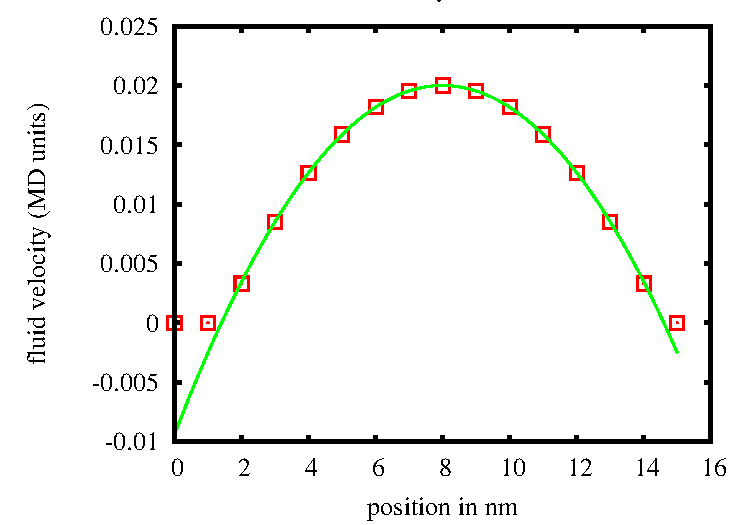
\includegraphics{../figs/poisseuille.pdf}
  \end{center}
  \caption{Poisseuille Flow in a slit Geometry.}
\end{figure}

\section{Constraints in \ES{}}
The \lstinline|constraint| command of \ES{} creates walls in the system.
They have a particular ``particle'' type and interact with the particles
present in the system with the potential defined 
between them. This means the distance
of every particle to the constraint is calculated and used as the distance 
in the interaction potential.

To set up a planar channel like the LB channel before one would use the commands:
\begin{lstlisting}[numbers=none]
constraint wall dist 0.5 normal 1. 0. 0. type 1
constraint wall dist -8.5 normal -1. 0. 0. type 1
inter 0 1 lennard-jones 1. 1. 1.225 0.25 0
\end{lstlisting}
This wall is felt only by particles of type 0 and has an effective width
of 6, as the potential goes steeply up at positions $x=1.5$ and $x=7.5$.

The syntax of the wall constraint looks weird at first, because a negative
distance from the origin (first argument) is given, but the idea is that
this distance times the normal vector is a point of the plane. For inclined
walls this syntax is more easy to understand.

\ES{} complains every time a particle penetrates the wall, as it does not
expect the particles to do so. This should normally cause no problem. 

To set up a system we have, of course to make sure, that our initial
configuration obeys the constraints. The easiest thing is to 
generate particle configurations randomly and repeat this process
for every particle until a configuration is found, that
is within the allowed range. Look at the script \lstinline|boundaries.tcl|
and see how that is solved. What does the script do?

\section{Simulating EOF in \ES{}}
The last thing that is missing for the simulation of EOF is
how to create a charged wall. This can be done with
particles, using the \lstinline|fix| command. The command
\begin{lstlisting}[numbers=none]
part 0 pos 1. 1. 1. q 1. fix 1 1 1
\end{lstlisting}
create a particle at the position $\left(1,1,1\right)$ with
charge 1 that is fixed in all the spacial dimensions.

In \lstinline|eof.tcl| two walls are created. Now use the material
from the other two scripts to run the final system.
Our we want to obtain a 10 Nanometer wide channel centered
$x=7.5$
\begin{enumerate}
  \item Create constraints at $x=1.5$ and $x=13.5$ and create 
    a particle-wall interaction. How can you assure that the 
    particles creating the wall charges are not affected by 
    interaction potential.
  \item
Use the particle
creation method from \lstinline|boundaries.tcl| to
create particles in the system. Create a repulsive potential between them.
  \item
Charge the particles so that
the overall system is neutral. 
  \item Add an electrostatic interaction with a Bjerrum length 
    of 0.7 (the room temperature Bjerrum length of water in nanometer).
  \item First do not exert an external force on the particles.
       Use a Langevin thermostat to bring the system to equilibrium.
       It will take some time for the ions to move towards the charged
       walls. You can use vmd to look see the process.
  \item
       Use the density profile method from \lstinline|boundaries.tcl|
       to determine the ion concentration profile. How many samples
       do you need to get a reasonable concentration profile.
   \item
     Plot the concentration profile with gnuplot. Compare with the
     the Poisson-Boltzmann result. 
   \item 
     Introduce an LB fluid with planar walls boundaries at 2.5 and 12.5. 
     Do not forget to remove the
     external force if you copy\&paste from \lstinline|poisseuille.tcl|.
   \item 
     Add an external force of 0.1 to all particles that do not form the
     charged wall in $y$-direction. Now run the system for enough time
     steps to get a good flux and velocity profile.
   \item 
     Finally calculate the velocity profile. You will have to 
     average over several steps. Keep in mind that number crunching
     with tcl is slow and that you will not need to average over too 
     many samples.
   \item 
     Compare the flux and velocity profiles with the result from
     theory. Do they agree?
   \item
     Now increase the charge density on the walls. Can you observe differences
     between theory and Computer simulations? They will likely be caused
     by the fact, that MD simulations of explicit ions automatically
     take into account ion correlations and the effect of the finite size
     of ions.
\end{enumerate}
















\bibliographystyle{unsrt}
\bibliography{refs}
\end{document}

